\chapter{Design}
Calculating a solution for a specific scenario is split into two parts. At first the underlying connection topology is determined.
Subsequently a channel assignment is computed for this specific topology. As input we expect a connected, undirected, weigthed graph.
  \begin{figure}[htbp]
    \centering
    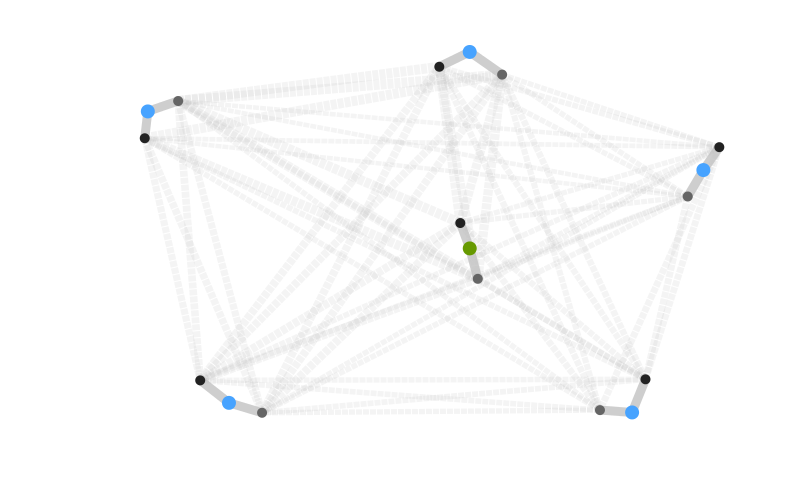
\includegraphics[width=1\columnwidth]{figures/graphseen.png}
    \caption{Graph representation of a scenario with 6 APs and 2 modules each. The grey eges indicate possible connectivity between the 
    modules. Edge weight(SNR) is mapped to edge thickness.}
    \label{fig:graphseen}
  \end{figure}
\section{Topology Creation}
  \subsection{Minimal/Optimal Spanning Tree Topology}
  In order to select those edges we want to use for creating connections between the APs, we use a derivation of the dijkstra algorithm. (cite dijkstra)
  We start by selecting an arbitray initial node and marking it as visited. All edges from this set of visited nodes to unvisited nodes are called productive edges.
  We keep those productive edges in a list sorted by their scores. The score of an edge is determined by the following formula:
  \begin{equation}
    ES=\frac{b}{(i + 1 )* c}
  \end{equation}
  where \textit{ES} is the Score of this Edge, \textit{b} is the expected bandwidth, \textit{i} is the number of interfering modules and \textit{c} is the connected count of the corresponding nodes.
  \begin{description}
    \item[Expected Bandwidth]
    describes the expected available bandwidth we assume to get for this link depending on the Signal-to-Noise-Ratio.
    For a given Signal-to-Noise-Ratio we can estimate the maximal possible thoughput.
    The bandwidth was chosen as the numerator, since it is effectively shared by those the radio modules within range.
    As we can see from the diagram, a higher SNR value results in more bandwidth available and works in favor of this edge.
    \item[Connected Count]
    Number of nodes we can reach from Module A and Module B by just using module-module edges. 
    A higher connected count diminishes the importance of this edge, since this value controls how many channels we can use later for the overall graph.
    If this value would not be taken into consideration for calculating the score, the algorithm would rather create long chains of connected modules. 
    Those links in this chain would admittedly have the best SNR values, but since they have to share the same channel, it would result in lowering the overall throughput.
    Granting this value a higher impact in the formula, like for example in 
    \begin{equation}
      ES=\frac{b}{(i + 1)* c^2}
    \end{equation}
    , would have the effect of overemphasizing 
    the channel distribution and lead to poor choices in links with respect to SNR - lowering overall throughput again.
    This simple, linear impact in the formula has been shown to achieve the best tradeoff between those two extremes.
    \item[Interfering Modules]
    Since the channel assignment has not taken place yet, we do not know which modules are actually interfering with this link if we would use it.
    However we do know to which other modules this module already has connections to and since those have to use the same channel in order to communicate with each
    other, we can derive an estimate as lower bound for the number of interfering modules for this link (A,B) by counting the following modules:
    Total Interfering Modules = Number of visited nodes which we can reach by one hop over a module-module connection from node A and B
    . Those modules definetly interfer with our current connection, since they:
      are in range with at least one node of this connection (one hop distance)
      have to use the same channel (communication over module-module link)
      do actually interfere, because we already decided to use this connection (visited node)
    The value is incremented by one, because if this connection would be used, itself again acts as a source for interference.
    With an increasing count in interfering modues, the value of the link decreases and vice versa. This reflects perfectly the concept of a shared medium.
  \end{description}
  For each round we determine from this list the edge with the highest score and mark the new node as visited and add also the new links to the list.
  Finally we have to update the scores for each affected link and continue with the next round until all nodes are marked visited.
  The outcome is a minimal spanning tree for this graph with a custom evaluation function.
  \subsection{Survival Path}
  Since a spanning tree is very susceptible to graph partition by just removing or failing one link we have to add redundant connections.
  Those redundant connections have to be carefully chosen in order not to negatively impact the successive channel assignment and neither to push interference.
  We accomplish this by iterating over all the edges of the spanning tree and simulate each connection failing. We then check if there is still exists 
  a path from Node A to Node B of this failing connection. Only if there is no path to the other node, we separate the nodes into two groups:
  The nodes we can reach from node A become group A and those nodes we can reach from node B become group B.
  Notice, that we do not have to separate the nodes into device and modules for the process of reconnection.
  We create a list with unused edges which connect the two groups and calculate the scores on them and pick again the edge with the highest score.
  This edge is, considering to the formula, the best edge to reconnect the two parts shall be known as part of the survival path.
  Nevertheless we have to be aware that it might not be feasible to reconnect those parts if the underlying structure does not permit it.
  This results in a robust network topology, which yields a high overall throughput.
  \begin{figure}[h]
    \centering
    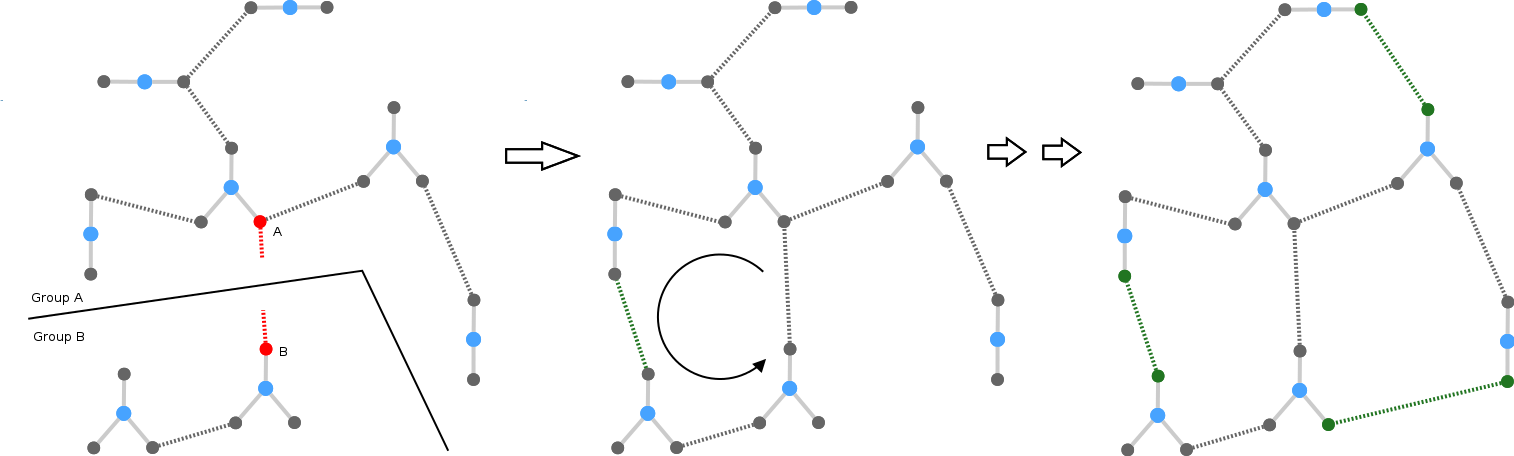
\includegraphics[width=1\columnwidth]{figures/survival_algo}
    \caption{Finding survival paths. Simulation of connection between node A and node B failing, creating two groups.
    Finding a survival path for node A and B. Eventually all connections have a survival path.}
    \label{fig:survival_algo}
  \end{figure}
  The survival path atribute for a graph can be expressed ind the following way:
  For each edge (a,b) of the calculated spanning tree graph G', find a path from a to b without traversing (a,b), 
  in a way that the the sum of the Edgescores of the path is maximal.

\section{Channel Assignment Algorithm}
  For a given network topology graph and a set of channel to chose from, we can now assign channels to the module-nodes. Therefore we iterate over all 
  edges and assign channels to the adjacent module-nodes if they do not already have one assigned. The channel for an edge, 
  or its corresponding module-nodes is chosen by the following pattern:
  Select all the modules which are connected by module-module edges. This set of nodes is called the channel-group. //explain the channel-list better//
  For all neighbouring modules which are not part of this group, if those modules have channels assigned to them, 
  increase the counter for this channel in the channel-list by one. At the beginning of the selection-process for a channel-group, the channel-list contains
  all available channels and their corresponding counter is set to 0.
  If all the modules have been processed, the channel-list shows us the local utilization of each channel which would lead to interference.
  From this list we pick those channels which have been used the least. If two or more channels are tied even on occurences, we select those channels which have
  been used the least in the overall graph. As a last resort if this still gives us more than one channel, we select one at random.
  Note that we can beyond respecting our own channel allocations in the channel-list also take those modules with their channels into consideration, 
  which are not part of our network - i.e. foreign radio modules. This allows us to even better adapt to the local environment and lets us for example
  avoid using heavily utilized channels like 1,6 and 11 in the 2.4Ghz Band if possible.
  The designated channel will then be assigend to all module nodes in the channel-group.
  \begin{figure}[h]
    \centering
    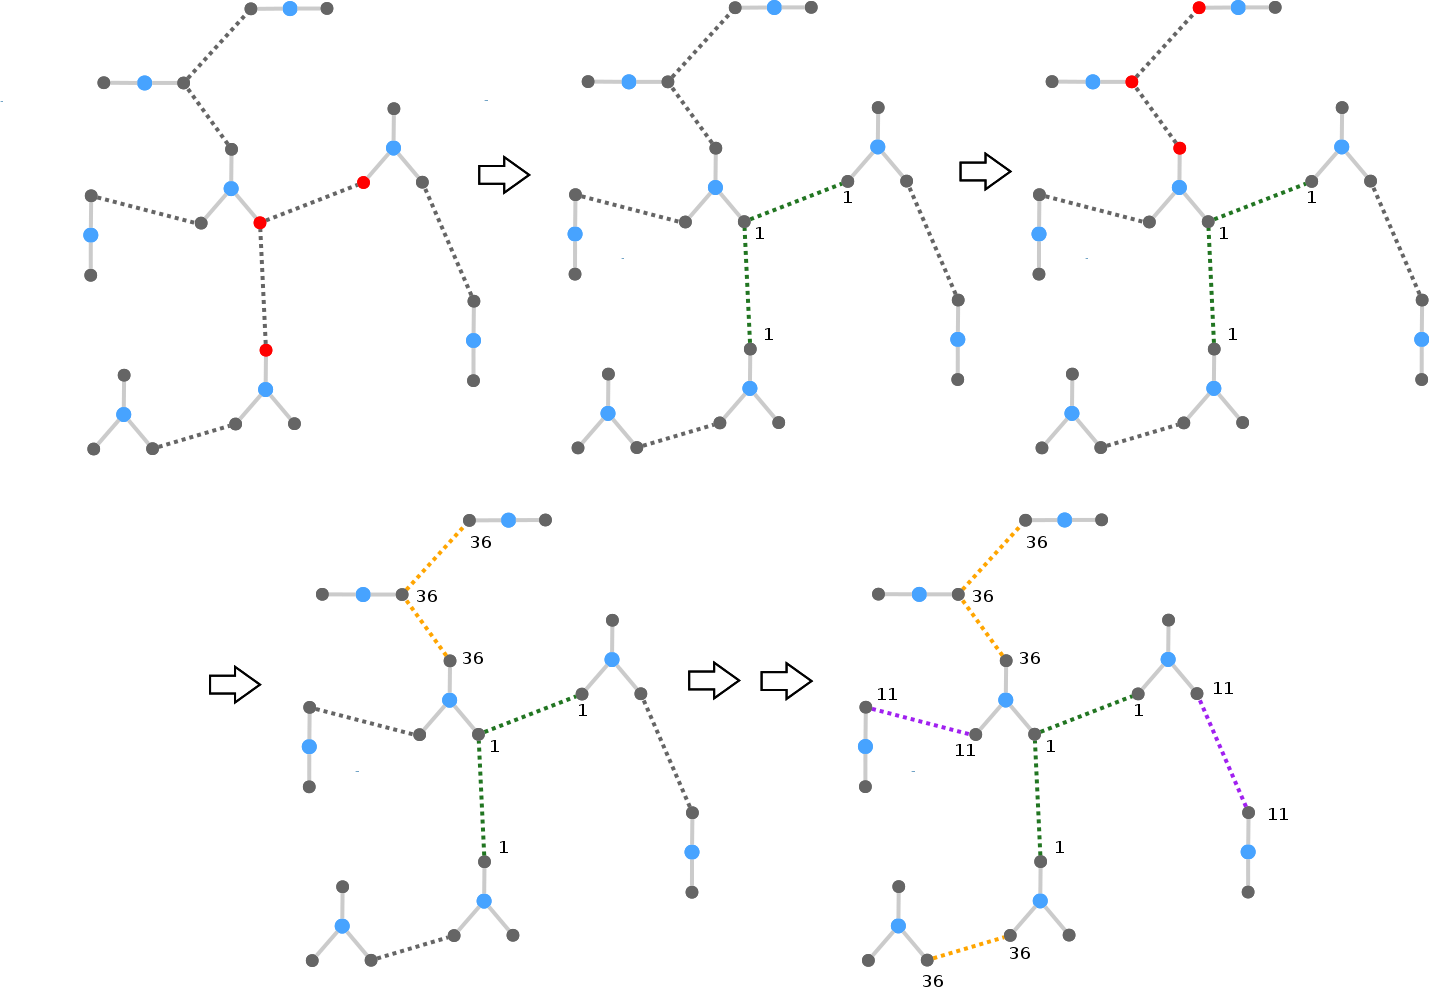
\includegraphics[width=1\columnwidth]{figures/caa_algo}
    \caption{Example channel assignment for a network with 8 Accesspoints with 2 and 3 modules equipped and available channels [1,11,36]. 
    The first four graphs represent the first 4 rounds. Red marked nodes represent a channel-group.}
    \label{fig:caa_algo}
  \end{figure}
